%%% LaTeX Template: Article/Thesis/etc. with colored headings and special fonts
%%%
%%% Source: http://www.howtotex.com/
%%% Feel free to distribute this template, but please keep to referal to http://www.howtotex.com/ here.
%%% February 2011
%%%
%%% Last updated September 2018 by CDM

%%%  Preamble
\documentclass[11pt,letterpaper]{article}
\usepackage[margin=1.0in]{geometry}
\usepackage[T1]{fontenc}
\usepackage[bitstream-charter]{mathdesign}
\usepackage[latin1]{inputenc}					
\usepackage{amsmath}						
\usepackage{xcolor}
\usepackage{cite}
\usepackage{hyphenat}
\usepackage{graphicx}
\usepackage{float}
%\usepackage{subfigure}
\usepackage{subfig} % Joe changed this
\usepackage{sectsty}
\usepackage[compact]{titlesec} 
\usepackage[tablegrid]{vhistory}
\allsectionsfont{\color{accentcolor}\scshape\selectfont}

%%% Definitions
\definecolor{accentcolor}{rgb}{0.0,0.0,0.5} 
\newcommand{\teamname}{Team 5}
\newcommand{\productname}{Jenga Playing Robot}
\newcommand{\coursename}{CSE 4316: Senior Design I}
\newcommand{\semester}{Fall 2018}
\newcommand{\docname}{Project Charter}
\newcommand{\department}{Department of Computer Science \& Engineering}
\newcommand{\university}{The University of Texas at Arlington}
\newcommand{\authors}{Joe Cloud \\ Gabriel Comer \\ Carlos Crane \\ Sammy Hamwi \\ Maxwell Sanders}

%%% Headers and footers
\usepackage{fancyhdr}
	\pagestyle{fancy}						% Enabling the custom headers/footers
\usepackage{lastpage}	
	% Header (empty)
	\lhead{}
	\chead{}
	\rhead{}
	% Footer
	\lfoot{\footnotesize \teamname \ - \semester}
	\cfoot{}
	\rfoot{\footnotesize page \thepage\ of \pageref{LastPage}}	% "Page 1 of 2"
	\renewcommand{\headrulewidth}{0.0pt}
	\renewcommand{\footrulewidth}{0.4pt}

%%% Change the abstract environment
\usepackage[runin]{abstract}			% runin option for a run-in title
%\setlength\absleftindent{30pt}			% left margin
%\setlength\absrightindent{30pt}		% right margin
\abslabeldelim{\quad}	
\setlength{\abstitleskip}{-10pt}
\renewcommand{\abstractname}{}
\renewcommand{\abstracttextfont}{\color{accentcolor} \small \slshape}	% slanted text

%%% Start of the document
\begin{document}

%%% Cover sheet
{\centering \huge \color{accentcolor} \sc \textbf{\department \\ \university} \par}
\vspace{1 in}
{\centering \huge \color{accentcolor} \sc \textbf{\docname \\ \coursename \\ \semester} \par}
\vspace{0.5 in}
\begin{figure}[h!]
	\centering
   	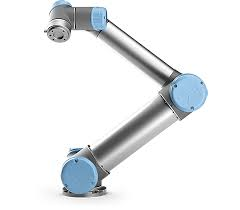
\includegraphics[width=0.4\textwidth]{images/ur5.jpeg}
\end{figure}
\vspace{0.5 in}
{\centering \huge \color{accentcolor} \sc \textbf{\teamname \\ \productname} \par}
\vspace{0.5 in}
{\centering \large \sc \textbf{\authors} \par}
\newpage


%\vspace{1 in}
%\centerline{January 13th, 2012}
%\newpage

%%% Revision History
\begin{versionhistory}
  	\vhEntry{0.1}{9.20.2018}{SH|JC|CC|MS|GC}{document creation}
  	\vhEntry{0.2}{9.28.2018}{SH|JC|CC|MS|GC}{document updates and draft 1 completion}
\end{versionhistory}
\newpage

%%% Table of contents
\tableofcontents
\newpage

%%% List of figures and tables (optional)
\listoffigures
%\listoftables
\newpage
\setcounter{table}{0}

%%% Agile project charter sections
\section{Vision}
The growing need for scientists, technologists, engineers, and mathematicians has led to much research on fostering interests in STEM at an early age. It has been shown \cite{McClure2017} that engaging younger students with demonstrations of science and technology correlates with future interest and success in STEM. Considering this increasing need and the recent decline in interest \cite{Sadler2012}, developing a playful demonstration targeted at younger audiences can help spurt new growth. This project serves as an interactive demonstration of computer science concepts with the goal of inspiring the next generation of scientists \& engineers.

%The Robot Jenga Player's vision is to show impressionable youth what they can achieve by pursuing an engineering degree. Displaying this project at different outreach and trade show events can give future engineers the ability to learn about, and use, the Jenga player. By showing them something enjoyable and interesting that can be achieved through an engineering degree, it may in turn spark an engineering curiosity that some of today's youth have. 

\section{Mission}
The objective of this project is to implement a Jenga-playing robot system involving a human opponent. Our solution will utilize 3D computer vision to develop scans of the tower's state, and a vacuum gripper to grip blocks. The human opponent will take turns with the robot performing block pulls and placing them at the top of the stack. The goal isn't necessarily to defeat the human opponent, but build a system capable of make multiple moves prior to the tower collapsing. 
\section{Success Criteria}
Upon completion of the computer vision aspect of our Jenga-playing robot prototype, we expect the following milestones to be met:

\begin{itemize}
  \item Ability to scan the collapsed playing field (unordered scattered blocks) in order to find the initial locations and orientations of the game pieces
  \item Ability to scan the vertical playing field and find changes between turns to create a map that will be used to determine the robot's next block pull
  \item Ability to recognize when the game has ended (blocks have collapsed)
\end{itemize}

\noindent
Upon completion of the UR-5 robotic gripper system, we expect the following milestones to be met:
\begin{itemize}
    \item Ability to grab and remove a block from any location in the vertical game field
    \item Ability to move and place a block into a c position
\end{itemize}

\noindent
Upon completion of the completed 3D-Vision and gripper systems, we expect the following milestones to be met:

\begin{itemize}
  \item Ability to algorithmically take blocks from the collapsed playing field and create the initial stacked game state
  \item A play time of less than 60 seconds per turn, which includes finding the most suitable block to remove using a custom game-play engine, removing the block, and stacking it on the top of the game field
\end{itemize}

\newpage

%%% Remaining project charter sections
\section{Background}
More than ever the need for engineers has increased. Society is moving towards automation and with it comes a need for engineers. To fill this need, it is the responsibility of engineers to attract the next generation of engineers to the field. One of the best way of attracting people to the profession is by building projects that people can see and experience. This is the basis for the Jenga playing robot.

The societal need for a Jenga robot is non-existent. We aren't designing this with the expectation of selling it for profit or creating patents (although, we aren't against these outcomes). Our intention for developing this robot is to create a robot that will entertain and interact with the public by playing the family-friendly game of Jenga.

Plenty of projects have been designed with the intention of swaying the opinions of the public towards engineering. There has been Rubik's cube solving robots, chess playing robots, and even other Jenga robots that have come before us. The goal of our project is no different from theirs, we plan on showcasing our robot to gain public interest for engineering rather than developing it for monetary gain. 

Our sponsor, Cloud9 Perception, is looking to build excitement for the engineering field as well as have a centerpiece to draw people into their conference booths. We will use their vision solutions and resources to help develop the robot to be able interact with conference guests. This interaction should be interesting enough to draw them into their booth and help bring them business as well as build awe towards engineering.

The Jenga Playing Robot has been done plenty of times before, but unlike our predecessors we intend to have the robot actually play with a player. The design of previous Jenga playing robots have the awe of a robot selecting from a tower of blocks correctly, but none before us have played Jenga against human opponents. We will surpass our predecessors by building a Jenga playing robot that is more robust and capable of competition.

\section{Related Work}
Our team found several implementations of Jenga playing robot arms that already exist, all of which were created for the purpose of academic research. However, these implementations would not be ideal for trade show demonstrations for various reasons, including lack of full automation, lack of interactivity, and excessive downtime between each round of play.

For instance, the Jenga playing manipulator created by Kroger et al. \cite{kroger2008manipulator} does not play against a human opponent. While their implementation was extremely successful in terms of the number of block pulls (the record highest tower was over 28 levels), for safety purposes, their implementation played against itself. This implementations goal was to stack the highest tower with no opponent. We would like for our implementation to play against human opponents in a controlled and safe manor.

Another implementation, created by Chia-Hung Lin \cite{lin2018robot} uses the same type of UR5 robotic arm as our project. However, Lin's project takes up to 60 seconds to scan the tower and make it's next move. Since our project is meant to be an exciting demonstration used to attract people at trade shows, we want to quicken the pace. Furthermore, Lin uses AR tags to mark important locations, like the edges of the tower. Since part of our goal is to demonstrate the capabilities of Cloud 9 Perception's vision hardware, we would like to avoid using AR tags, instead using computer vision to orient the robot around the tower.

The implementations by Kimura et al. \cite{kimura2010force} and Wang et al. \cite{wang2009robot} both use detailed physics simulations to decide which block to pull next. Their research could be quite useful when creating the algorithm that decides which block to pull next. However, in the case of Kimura et al., a human must assist the robot in pulling blocks by spinning a rotating platform that the Jenga tower rests on. While their implementation can nearly match average human players in number of block-pulls, this level of human assistance is not acceptable for our project. Our goal is to enable the UR5 Jenga playing robot to play a full game of Jenga against an opponent without assistance. In the case of Wang et al., they were able to detect movements in the tower that could lead to collapse, allowing them to rule out the more dangerous block pulls (in contrast to Kroger et al., who pulled blocks at random \cite{kroger2008manipulator}). However, their  This robot did not stack removed blocks on the top of the Jenga tower, and was therefore not a suitable opponent for a game of Jenga. 


%\newpage % Joe inserted, to make sure system overview has a sep page

\section{System Overview}
%Explain, at a high level, how you will implement a solution to the problem. Include a diagram of major components to the system (not a full architectural design, but a high level overview of the major system components and how a user or external system might interface). Avoid specific implementation details (operating system, programming languages, etc.). This section should occupy at least 1 full page.


The implementation of the Jenga Playing Robot depends on a few different technologies shown in the diagram below:

\begin{figure}[h!]
\centering
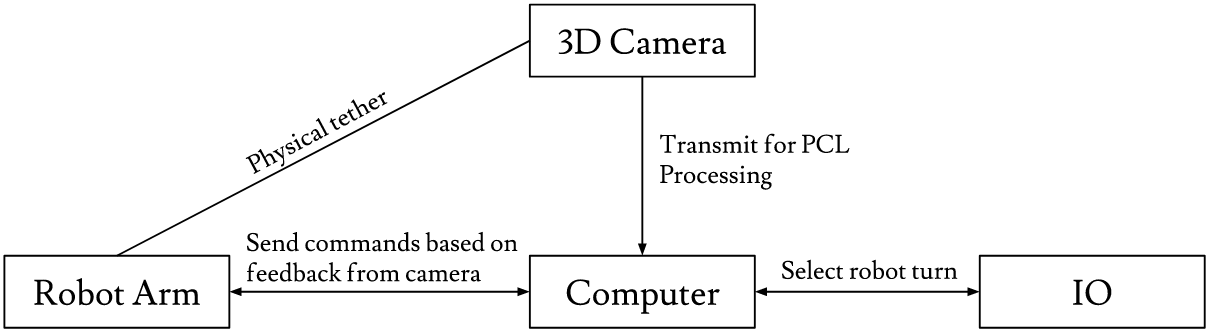
\includegraphics[width=0.8\linewidth]{images/sys_overview.png}
\caption{System Overview.}
\end{figure}

As shown in the diagram, our system consists of a UR5 robotic arm (with gripper), which is connected to a computer that handles the main processing, a 3D Camera to scan the playing field, and an IO interface to control the state of the game. This computer is responsible for tracking the state of the robot. This state can be defined as waiting for the human player to complete a turn, visually inspecting the stack for the next block pull, or performing a block pull and place based on the previously selected block. To accomplish this, the computer receives data from the camera (attached to the end effector of the robot), which is used during the scanning stage to determine the state of the Jenga stack. The state of the Jenga blocks can either be stacked or collapsed. When stacked, the goal is to find an available Jenga block, perform the pull and place, then wait for the human player to respond. In the case the Jenga stack is collapsed or collapses as a result of the robot's actions, the robot will clear a fixed playing zone of debris and begin re-stacking the blocks in place. The human opponents signals the robot via the IO interface when he or she has completed a turn.  

\begin{figure}[h!]
\centering
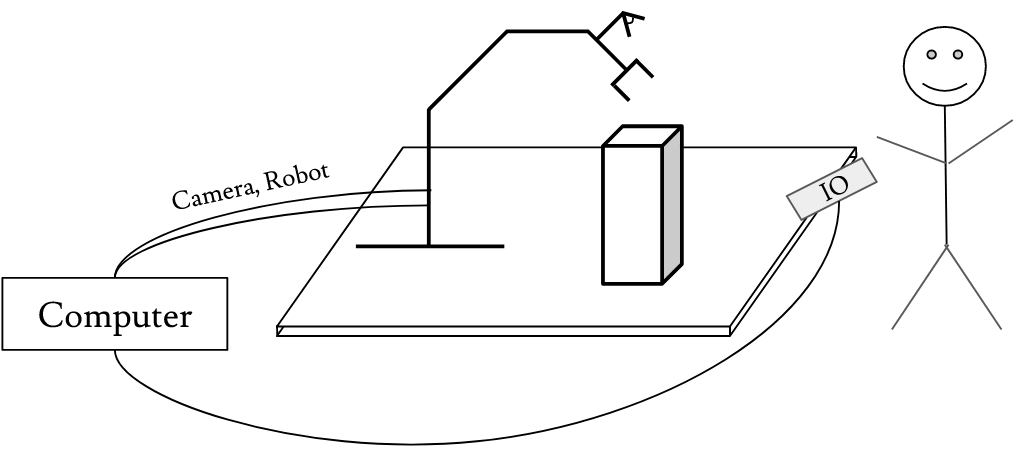
\includegraphics[width=0.78\linewidth]{images/system_setup.png}
\caption{Example Setup.}
\end{figure}
\section{Roles \& Responsibilities}
The stakeholders of the project will be our team, consisting of five members, who will be developing and seeing the project to completion. Cloud9 Perception, our sponsor, also has a stake in this project as they would like a product that showcases their 3D scanning technology and will be donating 3D scanning parts to this Jenga playing robot project. At a higher level, The University of Texas at Arlington has a stake in this project, as the success of the Jenga playing robot determines the preparedness of the students of the Department of Computer Science Engineering.

The point of contact for both our sponsor and our customer will be Dr. McMurrough, as the course professor and owner of Cloud9 Perception. We will be in contact with Dr. McMurrough in order to determine if we are going on the right path in developing the Jenga playing robot.

The team members consist of Gabe Comer, Carlos Crane, Joe Cloud, Sammy Hamwi, and Maxwell Sanders. Joe Cloud, being a computer engineer as well as experienced with robotics will be the lead on most of the hardware to software interface challenges that we will experience. Carlos Crane and Sammy Hamwi, having proficient front-end and user experience will be able to take charge of most of the user interface and design aspects of our project. Gabe Comer and Maxwell Sanders, along with Carlos and Sammy, will take care of 3D sensing, modeling, and algorithmic development of the gameplay and robotic arm interaction. Maxwell Sanders has had experience coding for the UR5 arm specifically, and will be the lead in developing that component.

Our team is going to rotate the product owner and the scrum master periodically. This will give all of us an opportunity at leadership as well as let us see the project from different roles and perspectives. 
\section{Cost Proposal}
This section contains the approximate budget for the project, where that money will come from, and any other support. This text should be replaced with a discussion and justification of major expenses, but not the actual monetary amounts (that will go in the preliminary budget section below). 
\begin{itemize}
    \item \textbf{Gripper}: One of the pivotal parts of the project is giving the robot the ability to actually interact with the tower. A proper gripper is worth the cost, since it is our only way for the robot to interact.
    
    \item \textbf{Camera}: The other pivotal part of the project. This gives our robot the ability to scan and analyze the tower. A Camera is necessary since without it the robot would be incapable of dynamic play.

    \item \textbf{Custom Jenga Tower}: A jenga tower that works for our project will likely have to be custom made. We would like to 3D print a tower ourselves so that we have control over the tower's specifications, which would be great since 3D printing would come at negligible cost to us. We would like to make slightly larger than usual blocks, with markings to easily distinguish the short and long sides of each block. The cost of a custom jenga tower should be less than \$100.
\end{itemize}
\subsection{Preliminary Budget}
\begin{table}[h!]
	\centering
	\begin{tabular}{|l|l|r|r|}
		\hline
		Category    &  Item                   & Quantity & Budget     \\
		\hline
        Gripper     & Robotiq Finger          &   1      & \$0-\$3000 \\
		Camera      & Intel Realsense / C9P   &   1      & \$0-\$150  \\
		Robot       & UR5                     &   1      & \$0        \\
  		Computer    & Intel NUC / NVIDIA TX2  &   1      & \$600      \\
  		Jenga Set   & Jumbo Jenga Extreme     &   1      & \$100      \\
  		IO          & Monitor                 &   1      & \$0-\$100  \\
  		            & KB/ USB Buttons         &   2      & \$0-\$10   \\
		\hline
	\end{tabular}
\end{table}

\subsection{Current \& Pending Support}
\begin{itemize}
    \item \textbf{CSE Department}: \$800 This is the default funding given to every Senior Design Project.
    \item \textbf{Cloud9 Perception}: \$? Dr. McMurrough has expressed interest in supporting this for trade show demonstrations.
\end{itemize}

\section{Facilities \& Equipment}
The main lab space to be used during the UR5 Jenga Playing Robot will be the Senior Design laboratory in the Engineering Research Building Room 208. We will use this space for accessing the UR5 robotic arm, 3D printing of components, and development and implementation of electronic components that will be programmed. 

Some specific equipment that will be used is as follows:
\begin{itemize}
    \item \textbf{UR5 Robotic Arm}: Leased from the College of Engineering at the University of Texas at Arlington
    \item \textbf{3D printers}: Such as UltiMaker2, FormLabs Form 2, and IIIP. Available for use at the Senior Design lab maker space
    \item \textbf{Laser cutter}: Available for use at the Senior Design lab maker space or the UT Arlington FabLab maker space
    \item \textbf{Soldiering equipment}: Available for use at the Senior Design lab maker space
    \item \textbf{Design software}:  For chip development, 3D printing. Available for use at the Senior Design lab maker space
\end{itemize}

Other spaces that may be used include the University of Texas at Arlington Library FabLab, which provides access to a workshop, laser cutter, and 3D printers. 
\section{Assumptions}
\begin{itemize}
    \item The UR5 Robotic Arm will be available for initial spec and testing by the second sprint cycle
    \item Funding and sponsorships will be secured for the computation, 3D sensing, and gripping components by the second sprint cycle
    \item The 3D sensing array will be available for development and testing by the third sprint cycle
    \item The robotic gripper will be available and/or developed by the third sprint cycle
    \item There will be ample power, lighting, and space available for the game to be played where it is going to be demonstrated
\end{itemize}
\section{Constraints}
The following list contains key constraints related to the implementation and testing of the project.

\begin{itemize}
  \item Final prototype demonstration must be completed by May 2019.
  \item The UR5 robot arm is currently being used by another Senior Design team, so we will have to share access to the arm.
  \item Total development costs, including purchasing cameras and grippers, must not exceed our budget of \$800 and support from sponsors.
  \item Since our project is meant to be used for demonstrations at trade shows, we may not be able to rely on consistent lighting conditions.
  \item The product must be easy to set up and interaction must be natural enough to be able to be demonstrated at trade shows.
\end{itemize}

\section{Risks}
The following high-level risk census contains identified project risks with the highest exposure. Mitigation strategies will be discussed in future planning sessions.

\begin{table}[h]
\resizebox{\textwidth}{!}{
\begin{tabular}{|l|l|l|l|}
\hline
 \textbf{Risk description} & \textbf{Probability} & \textbf{Loss (days)} & \textbf{Exposure (days)} \\ \hline
 UR5 Robot Arm out of order due to broken components  & 0.25 & 15 & 3.75 \\ \hline
 3D printed Jenga blocks do not work properly in game-play  & 0.20 & 8 & 1.6 \\ \hline
 Lack of required knowledge or skill in computer vision  & 0.50 & 10 & 5 \\ \hline
 Delays in shipping from overseas vendors  & 0.10 & 20 & 2 \\ \hline
 Late changes to project requirements & 0.15 & 18 & 2.7 \\ \hline
\end{tabular}}
\caption{Overview of highest exposure project risks} 
\end{table}
\section{Documentation \& Reporting}
%%% In this section, you will describe all of the various artifacts that you will generate and maintain during the project life cycle. Describe the purpose of each item below, how the content will be generated, where it will be stored, how often it will be updated, etc. Replace the default text for each section with your own description. Reword this paragraph as appropriate.

\subsection{Major Documentation Deliverables}

\subsubsection{Project Charter}
The Project charter is being maintained at a weekly basis. Our team meets at least once a week, every week. The designated meeting date is every Friday, but if more times needs to be allocated to the project then we may meet again. The initial version of the project charter will be delivered on October 1, 2018. The final version of the project charter will be delivered sometime in May 2019.

\subsubsection{System Requirements Specification}
The System Requirements Specification Documentation will be maintained at our weekly meeting. The team meeting for this specific document will only occur during it's designated sprint (Sprint 2). The SRS documentation will be updated under the circumstance of a system requirement being inadequately defined. The initial version will be delivered on October 23, 2018. The final version of the SRS documentation will be delivered sometime in May 2019.

\subsubsection{Architectural Design Specification}
The Architectural Design Specification Documentation will be maintained at our weekly meeting. The team meeting for this specific document will only occur during it's designated sprint (Sprint 3). If our team discovers faults in our design patterns, then we may have to update the architectural design specifications. The initial version will be delivered on November 13, 2018. The final version of the ADS documentation will be delivered sometime in May 2019.

\subsubsection{Detailed Design Specification}
The Architectural Design Specification Documentation will be maintained at our weekly meeting. The team meeting for this specific document will only occur during it's designated sprint (Sprint 4). If our team creates unique Jenga blocks, then we will have to update our DDS documentation with the correct drawings and dimensions of the blocks. The initial version will be delivered on December 04, 2018. The final version of the DDS documentation will be delivered sometime in May 2019.

\subsection{Recurring Sprint Items}

\subsubsection{Product Backlog}
Items will be added to our backlog when the SRS documentation is changed to specify new requirements. The backlog for this project is being shared with the collaborative platform Google Drive, using Google Sheets. Items in the backlog are being prioritized by team votes during our weekly meetings.

\subsubsection{Sprint Planning}
Each sprint is planned and documented during our team meetings. Using a sprint backlog chart, we can maintain and split the required work for a given sprint fairly between each team member. During SD1 there are 4 sprints, each being two weeks in length. 

\subsubsection{Sprint Goal}
Our team as a whole discusses and decides the sprint goal together. Our customer's, Dr. McMurrough, involvement was giving our team a project with the UR5 Robot Arm. Other than this involvement, our team decides the sprint goal.

\subsubsection{Sprint Backlog}
The product backlog items that make their way into the sprint backlog are decided as a team during our weekly team meetings. The backlog is currently maintained with the collaborative platform Google Drive, using Google sheets and Microsoft Excel.  

\subsubsection{Task Breakdown}
Individual tasks from the sprint backlog are assigned to a team member based on a combination of team decisions and voluntarily claim of the tasks. Time on each task are documented by the expected hours it will take and the actual hours the task took to complete. The sprint backlog is located in our teams Google Drive as a Google Sheets file.

\subsubsection{Sprint Burn Down Charts}
Our team as a whole is responsible for keeping up with, and maintaining, the burn down chart during each sprint. The burn down charts allows us to input the amount of time allocated to a task during a sprint, so that it will then automatically update the burn down chart. Doing this allows our team to view the progress made on the project during a given sprint. The burn down chart is located in our teams Google Drive as a Google Sheets file. (Refer to Figure 3)

\begin{figure}[ht]
    \centering
    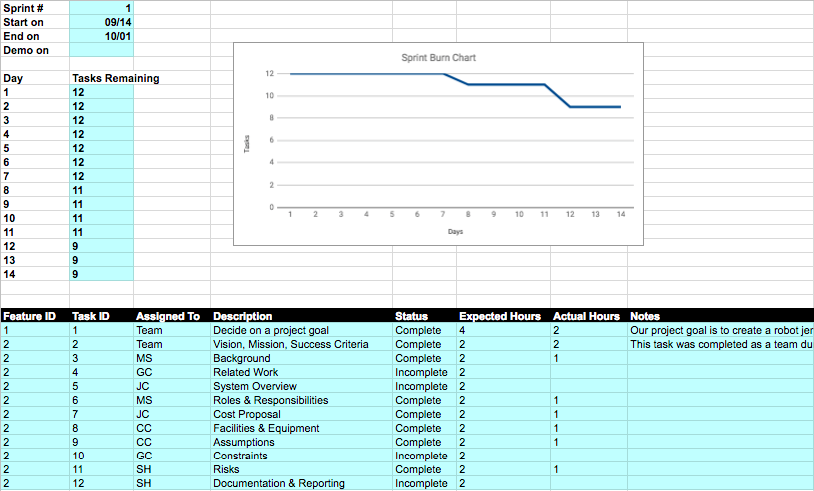
\includegraphics[width=1.0\textwidth]{images/sprint_burndown.png}
    \caption{Sprint burndown chart for Sprint 1}
\end{figure}

\subsubsection{Sprint Retrospective}
We will meet during the week between sprints and document in our engineering notebooks how the sprint went overall. We can also discuss what what we need to do better as a team.

\subsubsection{Individual Status Reports}
The individual status report will be completed every sprint week and discussed quickly at the weekly team meeting. We can fill out the individual status report in our engineering notebooks so we will have a record to improve upon.

\subsubsection{Engineering Notebooks}
We will fill out our individual status reports as well as any technical progress we have made in the engineering notebook. For accountability we will discuss our individual status reports at our weekly sprint meeting. We will also be able to sign the notebooks as witnesses during those weekly meetings as well.

\subsection{Closeout Materials}

\subsubsection{System Prototype}
Our system prototype will be to have a robot that will be able to scan the tower and play the game in favorable conditions for the robot. The robot will hopefully be able to get out of the lab and be demonstrated off-site. If we were to take it off-site to a conference which is the ultimate goal we need to make sure that it can handle playing against a human who doesn't know how the robot works.

\subsubsection{Project Poster}
Our project poser will be a 36" by 48" poster board that we will deliver near the final sprint to outline some of the features and development of our project. We may also have the robot out for an in-person demonstration.

\subsubsection{Web Page}
We intend to develop a simple webpage that states what our robot is capable of doing, who is on our team, the Doxygen documentation that we develop, and a link to Cloud9 Perception.

\subsubsection{Demo Video}
We will make a demo video displaying at least a part of a game that the robot will play. We will also produce plenty of B-roll footage throughout the semester that we can also upload and share to show the progress of the robot development.

\subsubsection{Source Code}
The source code will be maintained under a GitHub organization at https://github.com/jovialmcnulty. We will be adopting Git version control, in which the full source code of the project will be provided to the customer. We will be using a GNU 

\subsubsection{Source Code Documentation}
Code documentation will be done during code creation or as soon as possible after code creation. We will use Doxygen to generate our source code documentation, allowing us to provide that documentation in a browsable HTML file. 

%\subsubsection{Hardware Schematics}

\subsubsection{CAD files}
We will be designing our own set of Jenga blocks to be used by the UR5 Jenga playing robot. These blocks will be designed by our team and 3D printed. We will use Tinkercad to generate the model for an individual block. The model will be saved as an STL file. We will be using Cura to generate slices for the models, providing printable G-code.

\subsubsection{Installation Scripts}
We will provide a catkin package so the client can easily install the robot controls onto their own UR5 robot through ROS. The catkin package will include all dependencies for the robot setup, including drivers for the camera and gripper.

We will also include an installation script for the computer vision and user interface portions. These components will be installed using our installation script, and run on a PC that is working behind the scenes and providing vision and some control data to the robot.

\subsubsection{User Manual}
The UR5 Jenga playing robot will include a digital setup manual created using LaTeX. The setup manual will include instructions on how to setup the initial game state and game space markers. The manual will also describe how to calibrate the robot arm within the game space, and how to operate the user interface that controls when the robot takes its turn.

We will also include physical manuals that describe the rules for the game of Jenga, and how to play the game with the UR5 Jenga playing robot arm as your competitor. These physical copies of instructions are meant to be handouts used as part of the display, so that users interacting with the display will know the rules of the game.

\newpage

%%% References
\bibliographystyle{plain}
\bibliographystyle{reference/IEEEtran_custom}
\bibliography{reference/refs}{}

\end{document}